\documentclass[a4paper]{article}
\usepackage {changepage}
\usepackage{fancyhdr}
\usepackage {fontspec}
\usepackage {paralist}
\usepackage {multicap}
\pagestyle{fancy}
\setromanfont{Lantinghei SC Extralight}
\setmonofont{Courier New}
\XeTeXlinebreaklocale ``zh''
\XeTeXlinebreakskip = 0pt plus 1pt
\textheight = 650pt
\begin{document}
\title{实验报告 使用telnet发送邮件}
\author{姓名:王钦\quad 学号:13349112}
\date{}
\maketitle

\section*{ 实验目的}
\hangindent=4em \hangafter=-200{
	  \begin{itemize}
		\item 使用telnet 命令登录SMTP邮件服务器使用命令发送邮件
	  \end{itemize}
}
\section*{ 实验工具}
\hangindent=4em \hangafter=-200{
	  \begin{itemize}
		\item elementary luna OS base on ubuntu,Linux
		\item Gnome Terminal console
		\item Telent Command
	  \end{itemize}
}

\section*{ 实验流程}
\hangindent=4em \hangafter=-200{
	\begin{enumerate}
	\item 打开控制台输入\verb|telnet smtp.163.com 25|通过25端口登录163的邮件服务器
	\item 输入\verb|helo a|,a 是主机名,与163的邮件服务器打招呼
	\item 输入\verb|auth login|,登录验证用户名和密码,由于这里要求输入的是base64加密后的内容,先去百度找一个base64在线加密的网站把自己的163邮箱用户名和密码输入获取到加密后的用户名和密码并填入Terminal中。无误的话会提示\verb|Authentication successful|.
	\begin{center} 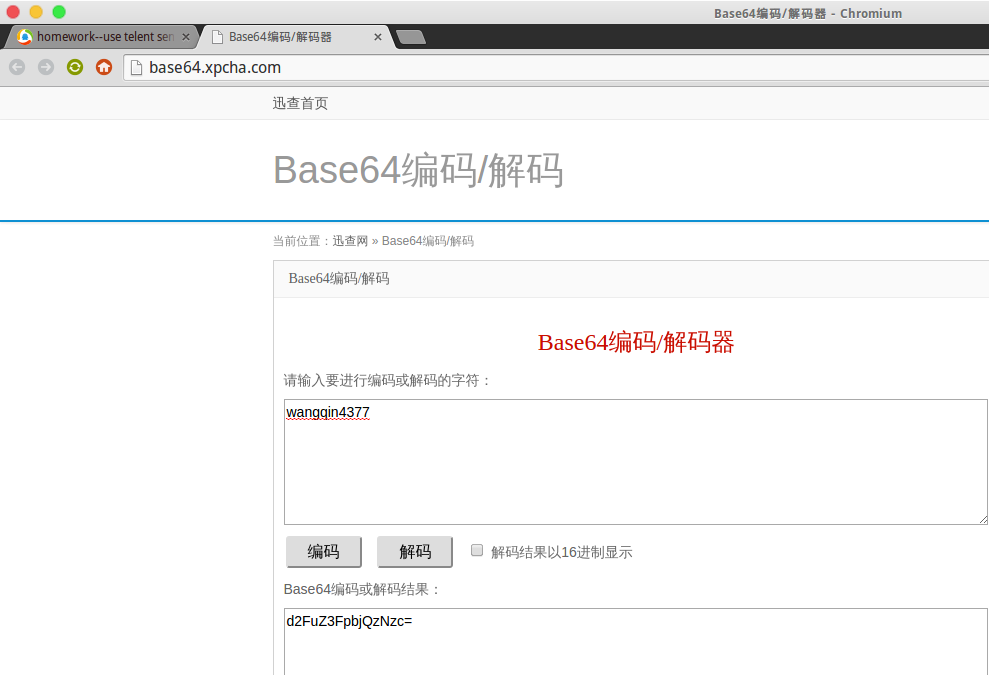
\includegraphics[scale=0.3]{Illustrations/base64.png} \mfcaption{base64 jiami}\end{center}
	\item 输入\verb|mail from:<wangqin4377@163.com>|,\verb|rcpt to:<admin@scientist2031.com>|,分别指邮件的发送者是\verb|wangqin4377@163.com|,接受者是\verb|admin@scientist2031.com|.
	\item 输入\verb|data|,开始输入邮件内容以.结束,subject表示主题,from是发件方,to是收件方,content是邮件正文.
	\begin{center} 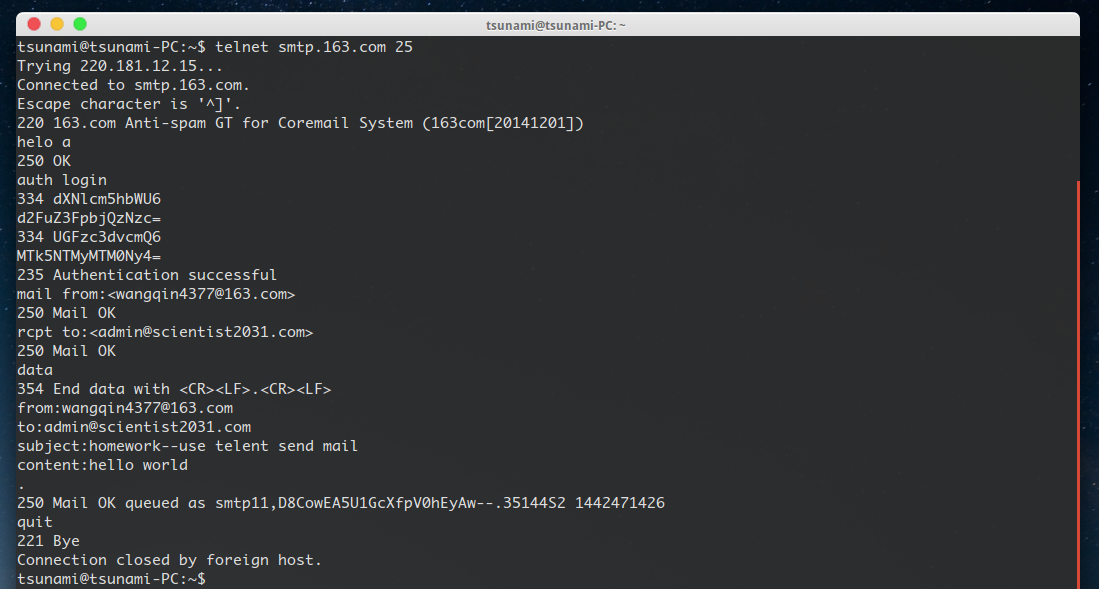
\includegraphics[scale=0.4]{Illustrations/console.png} \mfcaption{command}\end{center}
	\item 输入点后回车提示\verb|Mail OK|,发送成功。打开\verb|admin@scientist2031.com|的收件箱可以看到刚刚收到了一封通过telnet发送的邮件.
	\begin{center} 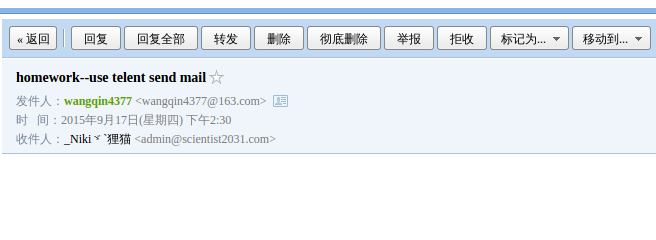
\includegraphics[scale=0.5]{Illustrations/mail.png} \mfcaption{result}\end{center}
	\end{enumerate}
\end{document}




